\chapter{Architecture and Design}

\pagebreak

\section{System Overview}

The system is designed in such a way that it contains three main modules:
\begin{itemize}
    \item User Interface
    \item Natural Language Processing
    \item Sentiment \& Keyword Extraction
\end{itemize}

\subsection{User Interface}

We’ve integrated the Facebook Messenger and Google Assistant interface to be able to get into an array of devices right away instead of marketing to install a new application. The benefits to this is that, we would not take up any extra space on the user’s phone and also that there are zero to none chances of being hacked or reverse engineered since everything is on the server side and not on the client side which is under user control.

\subsection{Natural Language Processing}

This happens in realtime as we are conversing with the chatbot. The sentences being sent to the NLP module are broken down and tokenized into various parts of speech tags. These help the model understand what the significance of each word means. We will then attempt to match the key word to one of the intents in our database through means of similarity. If there exists no such match, we will simply call the Default Fallback Intent and display to the user that it doesn’t know what to do.

\subsection{Sentiment \& Keyword Extraction}

In this phase, we attempt to summarize the journals written by the user and extract the sentiment of the message. This will explain a lot about the user’s intent and interests, not to mention the dislikes. This information can be stored for each individual user and later used in casual conversations.

\pagebreak

\section{Software Architecture}

First, architecture defines software elements. The architecture embodies information about how the elements relate to each other. This
means that it specifically omits certain information about elements that does not pertain to their interaction. Thus, an architecture is
foremost an abstraction of a system that suppresses details of elements that do not affect how they use, are used by, relate to, or interact
with other elements. In nearly all modern systems, elements interact with each other by means of interfaces that partition details about an
element into public and private parts. Architecture is concerned with the public side of this division; private details—those having to do
solely with internal implementation—are not architectural.

\subsection{System Block Diagram}

\begin{figure}[H]
    \centering
    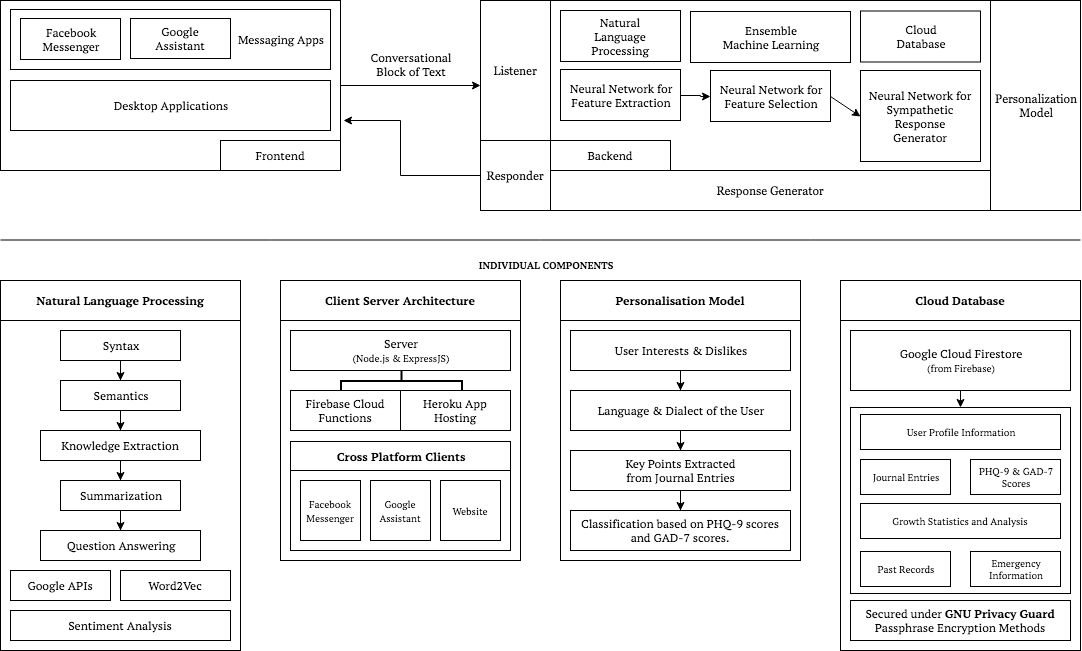
\includegraphics[width=\linewidth]{images/system-block-diagram.png}
    \caption{End-to-End System Block Diagram}
    \label{fig:system-block-diagram}
\end{figure}

\pagebreak

Second, the definition makes clear that systems can and do comprise more than one structure and that no one structure can irrefutably
claim to be the architecture. For example, all nontrivial projects are partitioned into implementation units; these units are given specific
responsibilities and are frequently the basis of work assignments for programming teams. This type of element comprises programs and
data that software in other implementation units can call or access, and programs and data that are private. In large projects, these
elements are almost certainly subdivided for assignment to subteams. This is one kind of structure often used to describe a system. It is
very static in that it focuses on the way the system's functionality is divided up and assigned to implementation teams.

\subsection{Inventive Steps}

\begin{figure}[H]
    \centering
    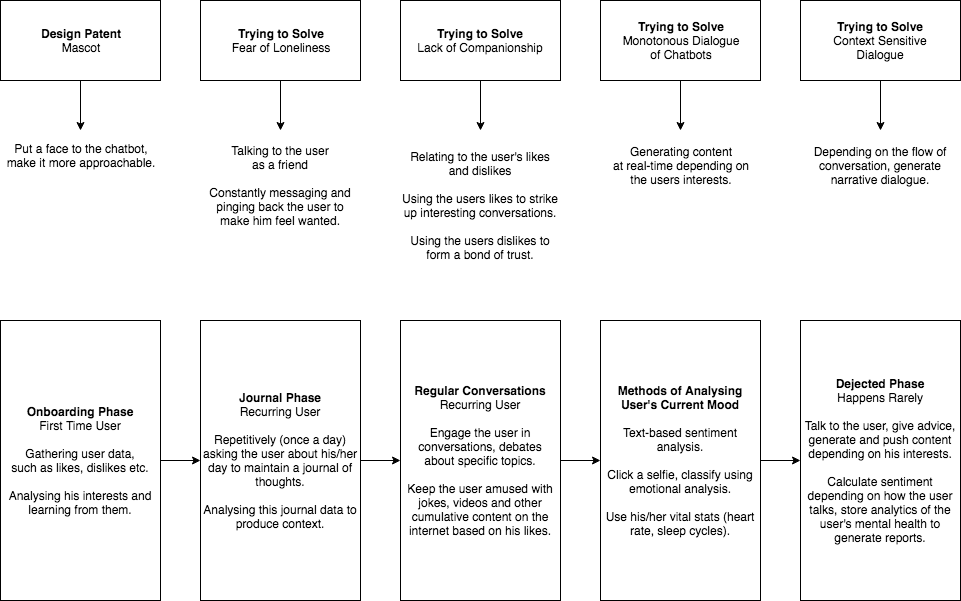
\includegraphics[width=\linewidth]{images/inventive-steps.png}
    \caption{Inventive Steps}
    \label{fig:inventive-steps}
\end{figure}

\subsection{Conversational Trees}

\begin{figure}[H]
    \centering
    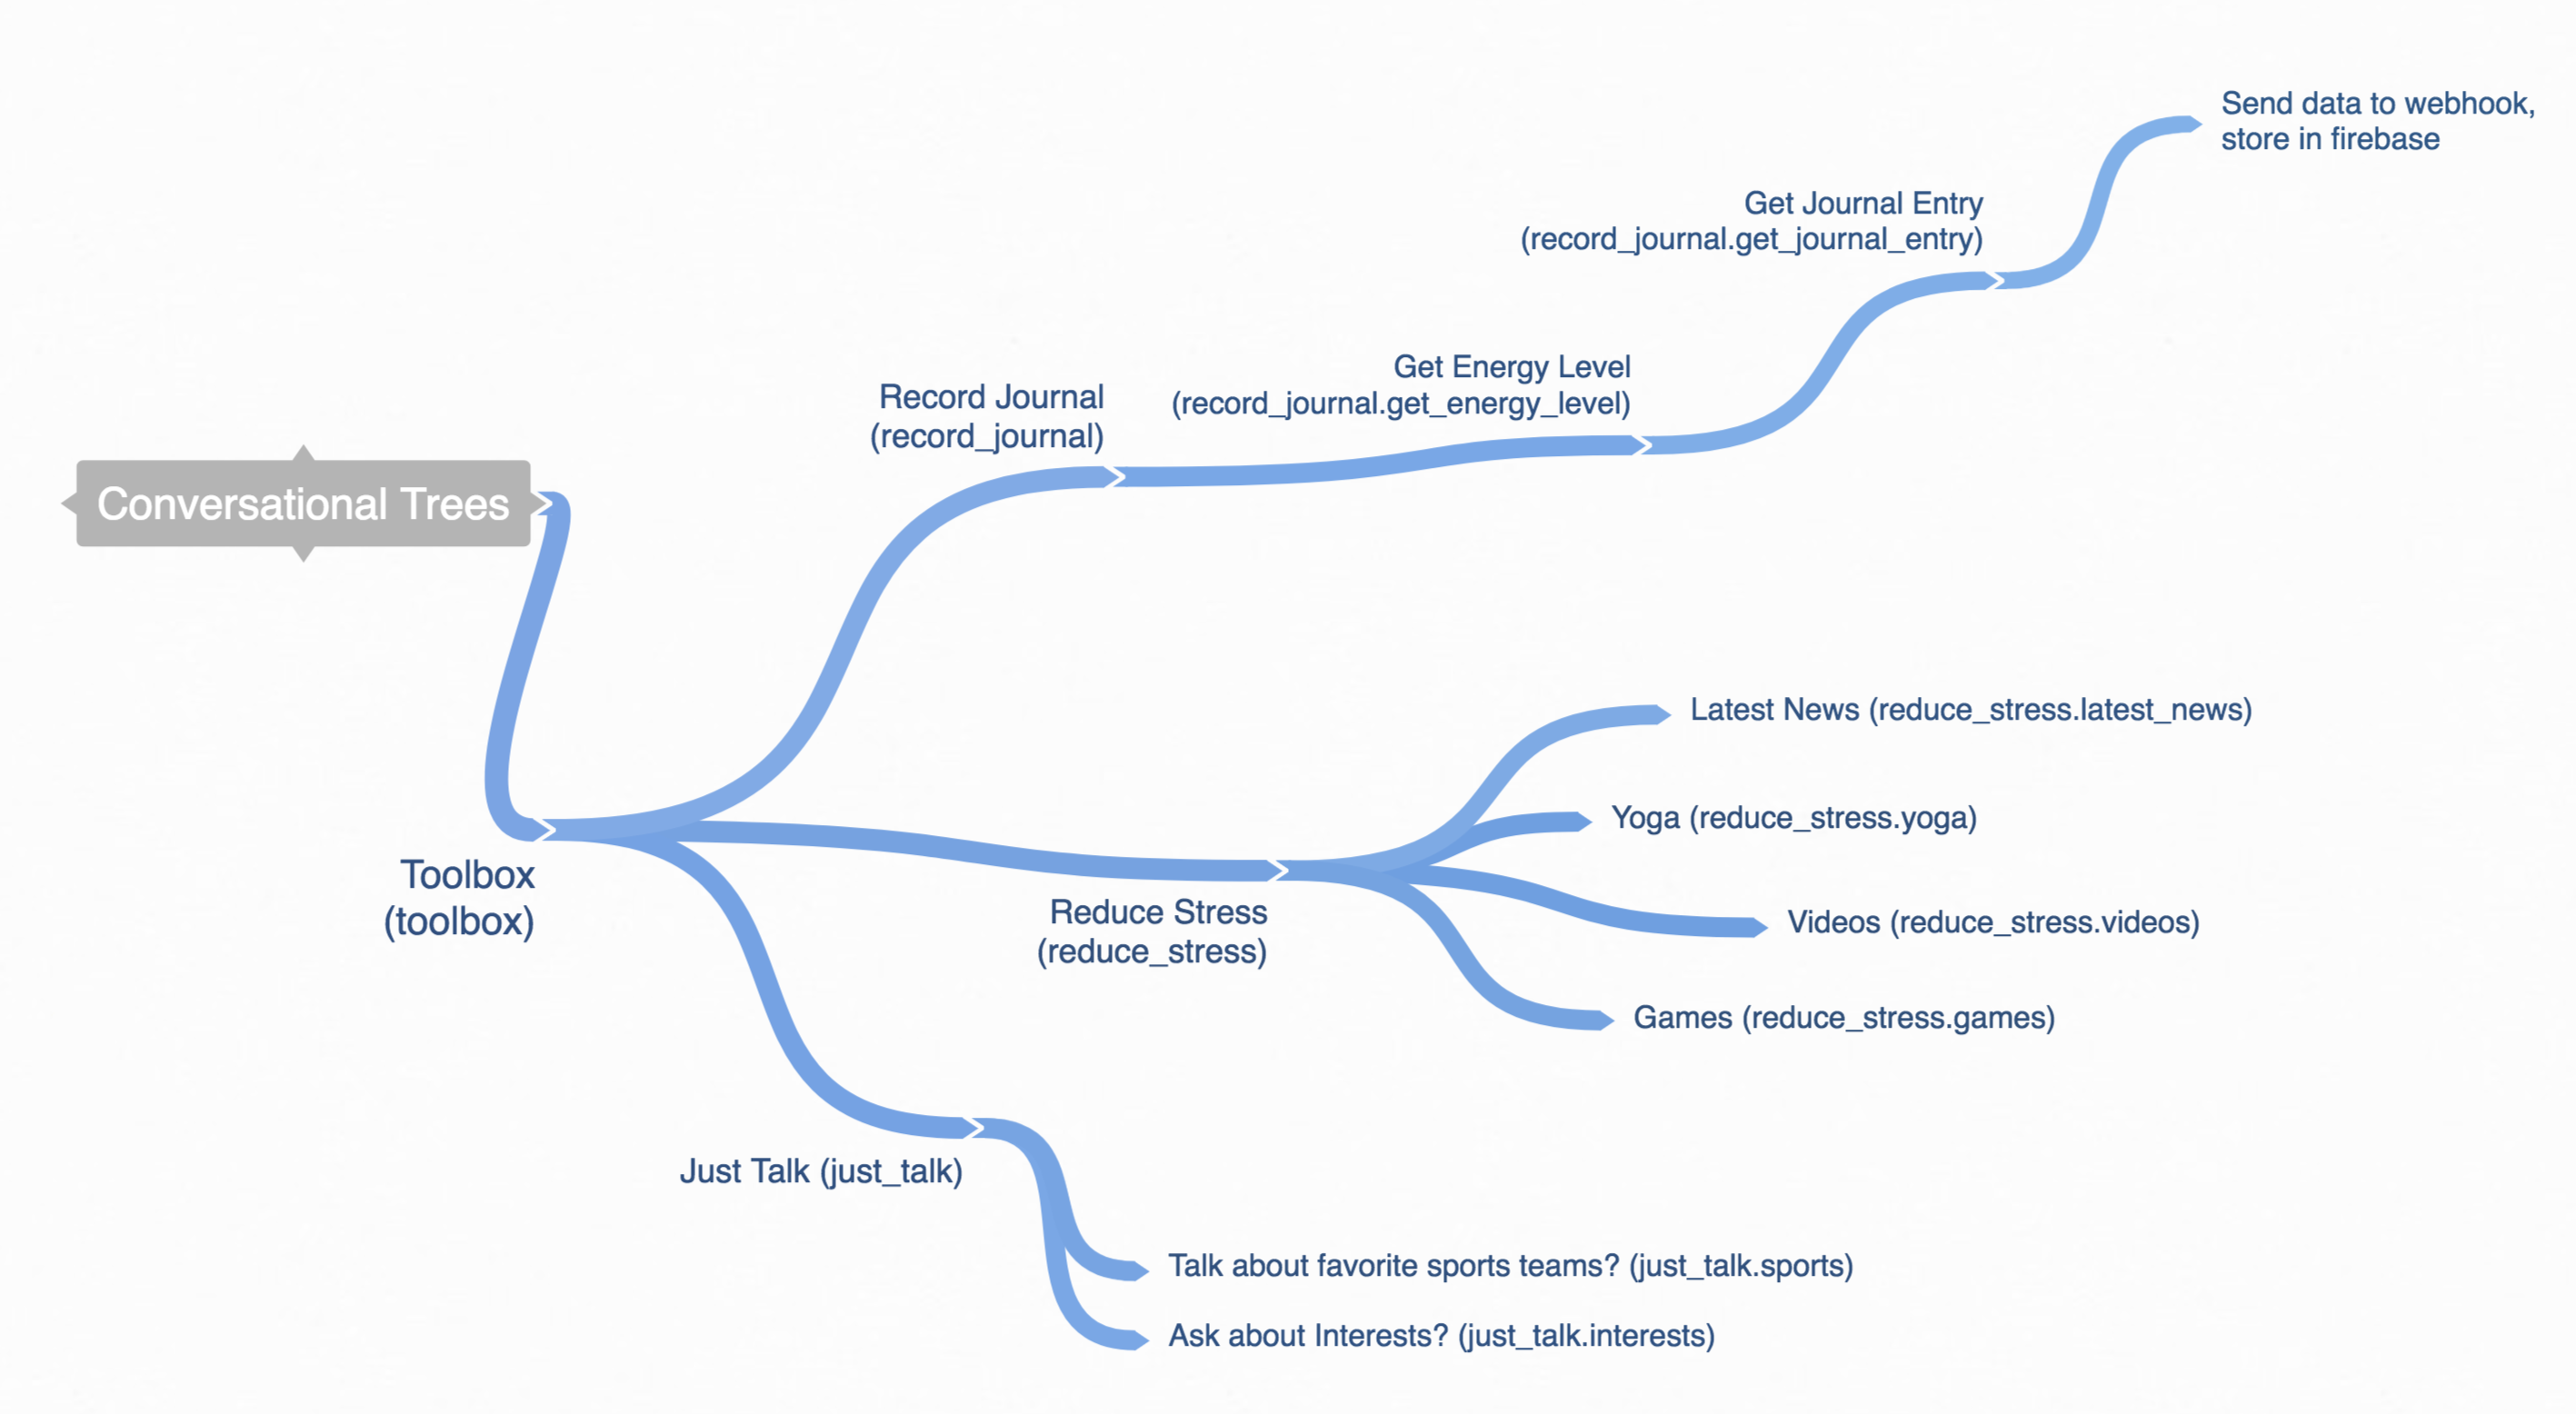
\includegraphics[width=\linewidth]{images/conversational-trees.png}
    \caption{Conversational Trees of the Chatbot}
    \label{fig:conversational-trees}
\end{figure}

\pagebreak

\section{Sentiment Analysis Anatomy}

VADER (Valence Aware Dictionary and sEntiment Reasoner) is a model that is used to predict the sentiment type and sentiment score of a particular sentence or a word input. It gives out an accurate score of each of the three sentiments - positive, negative and neutral. The reason for the preference of this tool compared to any other machine learning approach is the surpassing the complexity of a voluminous dataset. VADER has a Dictionary of lexicons that are used to predict the score of the sentences.

\begin{figure}[H]
    \centering
    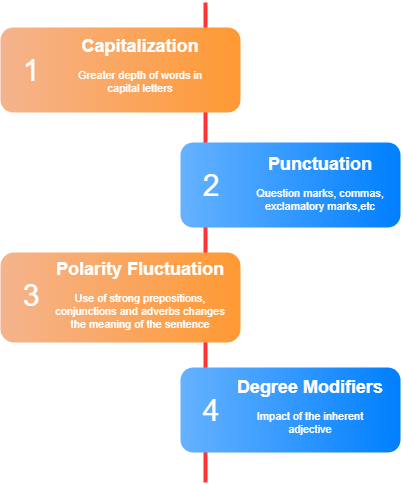
\includegraphics[width=10cm]{images/vader-model.png}
    \caption{Steps of the VADER Model}
    \label{fig:vader-model}
\end{figure}

\pagebreak

\section{Word2Vec (NLP) Structure}

Word2vec is a two-layer neural net that processes text. Its input is a text corpus and its output is a set of vectors: feature vectors for words in that corpus. While Word2vec is not a deep neural network, it turns text into a numerical form that deep nets can understand. Deeplearning4j implements a distributed form of Word2vec for Java and Scala, which works on Spark with GPUs. Word2vec’s applications extend beyond parsing sentences in the wild. It can be applied just as well to genes, code, likes, playlists, social media graphs and other verbal or symbolic series in which patterns may be discerned.

\begin{figure}[H]
    \centering
    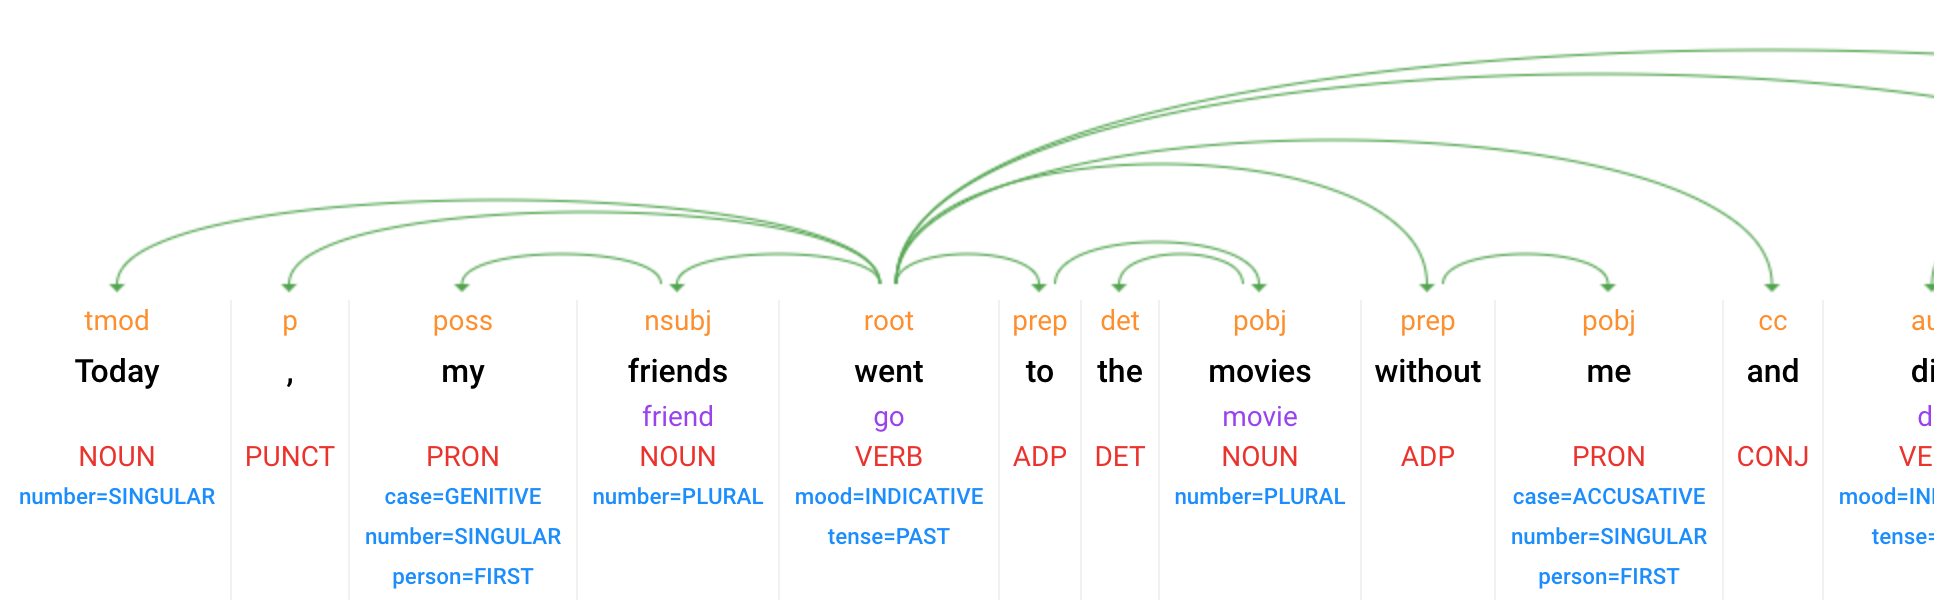
\includegraphics[width=\linewidth]{images/syntax-parsing.png}
    \caption{Syntax Parsing and Breakdown to Parts of Speech}
    \label{fig:syntax-parsing}
\end{figure}

Why? Because words are simply discrete states like the other data mentioned above, and we are simply looking for the transitional probabilities between those states: the likelihood that they will co-occur. So gene2vec, like2vec and follower2vec are all possible. With that in mind, the tutorial below will help you understand how to create neural embeddings for any group of discrete and co-occurring states. The purpose and usefulness of Word2vec is to group the vectors of similar words together in vectorspace. That is, it detects similarities mathematically. Word2vec creates vectors that are distributed numerical representations of word features, features such as the context of individual words. It does so without human intervention.

\begin{figure}[H]
    \centering
    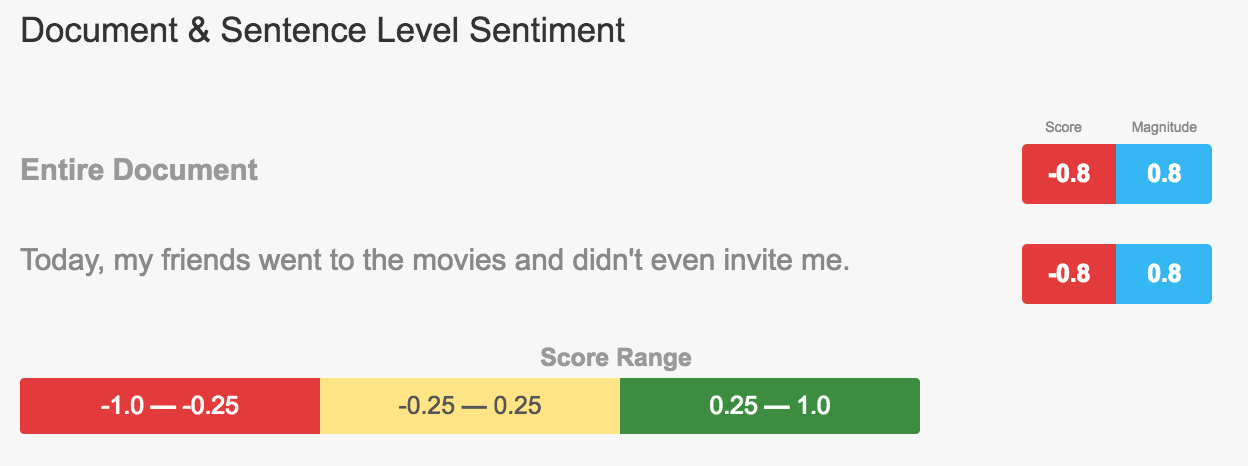
\includegraphics[width=\linewidth]{images/sentiment-analysis.png}
    \caption{Sentiment Analysis Response}
    \label{fig:sentiment-analysis}
\end{figure}

Given enough data, usage and contexts, Word2vec can make highly accurate guesses about a word’s meaning based on past appearances. Those guesses can be used to establish a word’s association with other words (e.g. “man” is to “boy” what “woman” is to “girl”), or cluster documents and classify them by topic. Those clusters can form the basis of search, sentiment analysis and recommendations in such diverse fields as scientific research, legal discovery, e-commerce and customer relationship management. The output of the Word2vec neural net is a vocabulary in which each item has a vector attached to it, which can be fed into a deep-learning net or simply queried to detect relationships between words.
